\documentclass{article}
% \documentclass[twocolumn]{article}
\usepackage{graphicx} % Required for inserting images
\usepackage{tikz} 
\usepackage{amsmath}
\usepackage{booktabs}

\newcommand{\mybox}[5]{
    \begin{center}
    \begin{tikzpicture}
        \node[anchor=text,text width=\columnwidth+1.0cm, draw, rounded corners, line width=1pt, fill=#3, inner sep=5mm] (big) {\\#4};
        \node[draw, rounded corners, line width=.5pt, fill=#2, anchor=west, xshift=5mm] (small) at (big.north west) {#1};
    \end{tikzpicture}
    % \caption{#5}
    \end{center}
}



\title{25.9.2 Snarkifying Mithiril}

\author{Wuyunsiqin \quad \quad Bingsheng Zhang \\ 
Zhejiang University, CHN \\
22521299@zju.edu.cn \quad bingsheng@zju.edu.cn}
% \date{May 20 2025}




\begin{document}

\maketitle

\section{Comparison with Jia Liu's work}

\begin{table}[htbp]
\centering
\caption{Comparison between our implementation and Jia Liu's work}
\label{tab:comparison}
\begin{tabular}{|c|p{5cm}|p{5cm}|}
\hline
\textbf{Aspect} & \textbf{Jia Liu's work} & \textbf{Our Implementation} \\
\hline
\textbf{Elliptic Curve} & Jubjub curve & BN254 curve \\
\hline
\textbf{Signature Scheme} & Modified into a \textbf{deterministic scheme}
 & Original \textbf{BLS signature} used in Mithril \\
\hline
\textbf{MSM Operation} & \textbf{MSM2 optimisation} (circuit layout modification to handle two multiplications at once, reducing rows per verification) & variable\_base\_msm\_custom function from halo2-lib \\
\hline
\textbf{Hardware Environment} & AWS instance r7i.12xlarge with 48 vCPU and 384GB memory 
 & Local server with 48-core Intel Xeon Silver 4214 CPU  and 128 GB memory\\
\hline
\end{tabular}
\end{table}



\begin{table}[htbp]
\centering
\caption{Certificate circuit with \textbf{msm2 optimisation}}
\label{tab:cert-msm2}
\begin{tabular}{|c|c|c|c|c|c|}
\hline
\textbf{Degree} & \textbf{Advice rows} & \textbf{Quorum\_max} & \textbf{Proving time} & \textbf{Peak memory} & \textbf{Verifying time} \\
\hline
11 & 1752 & 1    & 365.744ms & --    & 8.854ms \\
12 & 3240 & 2    & 549.739ms & --    & 7.696ms \\
13 & 7704 & 5    & 846.477ms & --    & 8.879ms \\
14 & 15144 & 10  & 1.517s    & --    & 9.482ms \\
15 & 31512 & 21  & 2.947s    & --    & 7.460ms \\
16 & 64248 & 43  & 6.057s    & --    & 7.782ms \\
17 & 129720 & 87 & 12.404s   & --    & 8.372ms \\
18 & 260664 & 175 & 25.135s  & 14GB  & 8.162ms \\
19 & 522552 & 351 & 50.860s  & 22GB  & 7.034ms \\
20 & 1046328 & 703 & 103.608s & 37GB & 7.063ms \\
21 & 2092392 & 1406 & 208.313s & 69GB & 7.582ms \\
22 & 4184520 & 2812 & 428.707s & 136GB & 8.300ms \\
\hline
\end{tabular}
\vspace{0.3em}

\footnotesize{Proving 2272 signatures (degree 22): proving time 415.945s, peak memory 136GB.}
\end{table}


\begin{table}[htbp]
\centering
\caption{Certificate circuit \textbf{without msm2 optimisation}}
\label{tab:cert-noms2}
\begin{tabular}{|c|c|c|c|c|c|}
\hline
\textbf{Degree} & \textbf{Advice rows} & \textbf{Quorum\_max} & \textbf{Proving time} & \textbf{Peak memory} & \textbf{Verifying time} \\
\hline
11 & --     & --   & --        & --   & -- \\
12 & 2264   & 1    & 434.322ms & --   & 6.853ms \\
13 & 6264   & 3    & 700.636ms & --   & 7.464ms \\
14 & 16264  & 8    & 1.437s    & --   & 6.578ms \\
15 & 32264  & 16   & 2.732s    & --   & 7.394ms \\
16 & 64264  & 32   & 5.397s    & --   & 7.476ms \\
17 & 130264 & 65   & 10.994s   & --   & 6.939ms \\
18 & 260264 & 130  & 21.930s   & 9GB  & 6.017ms \\
19 & 522264 & 261  & 44.785s   & 13GB & 7.571ms \\
20 & 1046264 & 523 & 90.909s   & 21GB & 6.969ms \\
21 & 2092264 & 1046 & 180.081s & 38GB & 6.758ms \\
22 & 4186264 & 2093 & 363.844s & 69GB & 6.961ms \\
23 & 8374264 & 4187 & 743.101s & 131GB & 6.838ms \\
\hline
\end{tabular}
\vspace{0.3em}

\footnotesize{Proving 2272 signatures (degree 23): proving time 581.347s, peak memory 135GB.}
\end{table}


\begin{figure}
    \centering
    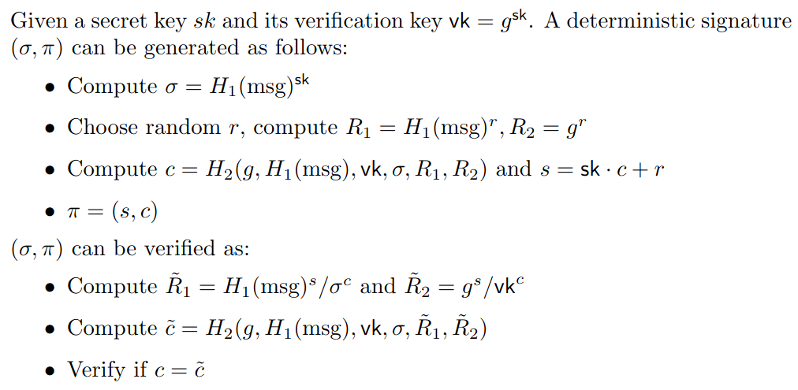
\includegraphics[width=1\linewidth]{21.png}
    % \caption{Enter Caption}
    \label{fig:placeholder}
\end{figure}
\begin{figure}
    \centering
    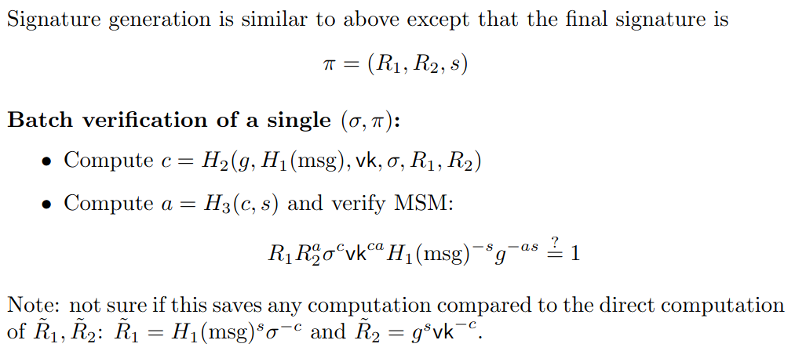
\includegraphics[width=1\linewidth]{23.png}
    % \caption{Enter Caption}
    \label{fig:placeholder}
\end{figure}
\begin{figure}
    \centering
    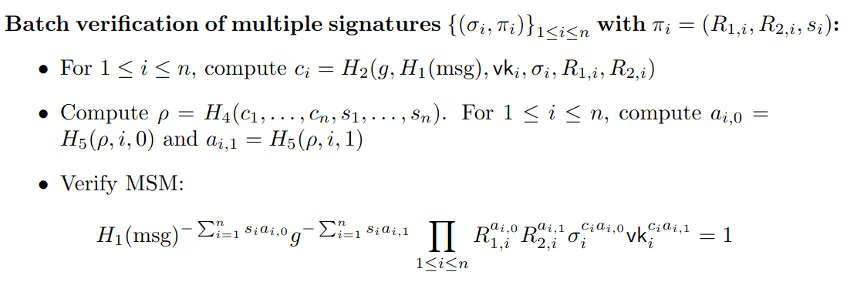
\includegraphics[width=1\linewidth]{24.png}
    % \caption{Enter Caption}
    \label{fig:placeholder}
\end{figure}

\newpage

\section{Snarkifying Mithril (Practical)}
\label{sec:snarkifying-mithril-practical}

This section implements a Halo2-based zero-knowledge cross-chain protocol instantiated with Mithril. The circuit covers: (i) unweighted BLS multisignature aggregation ($\mathsf{MSP.A}$), (ii) seed-weighted BLS aggregation ($\mathsf{MSP.B}$), (iii) lottery index range \& uniqueness checks, (iv) eligibility/threshold checks against stake, and (v) Merkle membership checks for registered signers. The experimental environment matches the previous section.

\subsection{Experimental Tasks}
\begin{itemize}
  \item \textbf{MSP.A (baseline aggregation).} Implements the straightforward BLS aggregation and in-circuit pairing check $e(\mu,g_2)=e(H_{\mathbb{G}_1}(\text{"M"}\Vert msg), ivk)$. We measure proving time, proof size, and verification time as the number of aggregated signatures grows.
  \item \textbf{MSP.B (seed-weighted aggregation).} Extends aggregation with per-signer short exponents $e_i \leftarrow H_\lambda(i,e_{\boldsymbol{\sigma}})$ and $(\mu,e_{\boldsymbol{\sigma}})$ where $e_{\boldsymbol{\sigma}}\leftarrow H_p(\boldsymbol{\sigma})$. The circuit proves the weighted pairing equation. We observe higher proving cost due to hashing and multi-scalar multiplications (MSMs) with weights.
  \item \textbf{Lottery index check.} Ensures $\mathsf{index}_i\!\le m$ for all $i$ and $\mathsf{index}_i\!\ne\!\mathsf{index}_j$ for $i\ne j$. The uniqueness constraint induces $O(n^2)$ comparisons; we report scaling behavior.
  \item \textbf{Eligibility/threshold check.} For each signer, enforces $ev_i=\mathsf{MSP.Eval}(\mathsf{topic},\mathsf{index}_i,\sigma_i)$ and $ev_i \le \phi(\mathsf{stake}_i)$. The circuit cost grows roughly linearly in the number of checked signers.
\end{itemize}

\subsection{Benchmark Tables}

\begin{table}[htbp]
  \centering
  \caption{MSP.A (unweighted aggregation) results}
  \renewcommand{\arraystretch}{0.9}
  \setlength{\tabcolsep}{10pt}
  \begin{tabular}{lcccccc}
    \toprule
    \textbf{aggregated signatures} & \textbf{2} & \textbf{200} & \textbf{2000} & \textbf{4000} & \textbf{6000} & \textbf{8000} \\
    \midrule
    Proving time (s)     & 19.17 & 29.51 & 72.89 & 123.67 & 181.38 & 226.84 \\
    Proof size (bytes)   & 3072  & 4128  & 11424 & 18944  & 26944  & 34944  \\
    Verification time (ms) & 20.93 & 9.09  & 19.95 & 16.03  & 20.25  & 55.16  \\
    \bottomrule
  \end{tabular}
  \label{tab:mspa_benchmark_en}
\end{table}


\begin{table}[htbp]
  \centering
  \caption{MSP.B (seed-weighted aggregation) results}
  \renewcommand{\arraystretch}{0.9}
  \setlength{\tabcolsep}{10pt}
  \begin{tabular}{lcccccc}
    \toprule
    \textbf{aggregated signatures} & \textbf{8} & \textbf{16} & \textbf{32} & \textbf{64} & \textbf{128} & \textbf{256} \\
    \midrule
    Proving time (s)     & 35.73 & 48.48 & 65.37 & 103.75 & 184.02 & 327.30 \\
    Proof size (bytes)   & 5856  & 7936  & 10944 & 17312  & 30240  & 55744  \\
    Verification time (ms) & 10.30 & 14.68 & 15.05 & 14.54 & 24.51  & 69.35  \\
    \bottomrule
  \end{tabular}
  \label{tab:mspb_benchmark_en}
\end{table}


\begin{table}[htbp]
  \centering
  \caption{Lottery index check results (range \& uniqueness)}
  \renewcommand{\arraystretch}{0.9}
  \setlength{\tabcolsep}{10pt}
  \begin{tabular}{lccccc}
    \toprule
    \textbf{indices} & \textbf{128} & \textbf{256} & \textbf{512} & \textbf{1024} & \textbf{2048} \\
    \midrule
    Proving time (s)     & 4.08 & 6.77  & 13.41 & 37.39 & 122.49 \\
    Proof size (bytes)   & 960  & 1920  & 4576  & 14944 & 14944 \\
    Verification time (ms) & 5.05 & 6.15 & 9.42  & 15.10 & 13.08 \\
    \bottomrule
  \end{tabular}
  \label{tab:index_check_benchmark_en}
\end{table}


\begin{table}[htbp]
  \centering
  \caption{Eligibility / stake-threshold check results}
  \renewcommand{\arraystretch}{0.9}
  \setlength{\tabcolsep}{10pt}
  \begin{tabular}{lccccc}
    \toprule
    \textbf{checks} & \textbf{128} & \textbf{256} & \textbf{512} & \textbf{1024} & \textbf{2048} \\
    \midrule
    Proving time (s)     & 10.14 & 12.78 & 17.36 & 26.39 & 44.56 \\
    Proof size (bytes)   & 1344  & 1920  & 2848  & 4800  & 8832 \\
    Verification time (ms) & 6.77  & 6.39  & 7.10  & 11.24 & 12.59 \\
    \bottomrule
  \end{tabular}
  \label{tab:eligibility_check_benchmark_en}
\end{table}


% \begin{table}[htbp]
% \centering
% \caption{Merkle membership proof results (transposed, with stake)}
% \renewcommand{\arraystretch}{0.9}
% \setlength{\tabcolsep}{8pt}
% \begin{tabular}{lccccccc}
% \toprule
%  & \textbf{16} & \textbf{32} & \textbf{64} & \textbf{128} & \textbf{256} & \textbf{512} & \textbf{1024} \\
% \midrule
% original proofs    & 32    & 64    & 128   & 256   & 512   & 1024  & 2048   \\
% Proving time (s)     & 5.68  & 7.60  & 13.44 & 23.29 & 48.63 & 100.05 & 213.25 \\
% Proof size (bytes)    & 704     & 1056    & 2112    & 3872    & 8448    & 17600    & 38016    \\
% Verification time (ms) & 6.57  & 4.47  & 7.64  & 8.13  & 11.65 & 13.61  & 20.31  \\
% \bottomrule
% \end{tabular}
% \label{tab:merkle_proof_benchmark_transposed}
% \end{table}




\newpage

\section{Snarkifying Mithril(Theoretical)}



\subsection{SNARK}
A SNARK for a relation $\mathcal{R}$ is a triple of PPT algorithms $\Pi = (\mathsf{Setup}, \mathsf{Prove}, \mathsf{Verify})$ defined as follows:


\begin{itemize}
    \item $  \mathsf{srs} \leftarrow \mathsf{Setup}(1^\lambda)$:On input security parameter $\lambda$
, it outputs a structured reference string $\mathsf{srs}$.   
    \item $\pi \leftarrow \mathsf{Prove}(\mathsf{srs}, x, w)$: On input $\mathsf{srs}$, a statement $x$ and a witness $w$ such that $(x, w) \in \mathcal{R}$, output a proof $\pi$.
    \item $0/1 \leftarrow\mathsf{Verify}(\mathsf{srs},x,\pi) $:On input $\mathsf{srs}$, a statement $x$, and a
proof $\pi$, it outputs either 1 indicating accepting the statement or 0 for rejecting it.
\end{itemize}

\subsection{BLS}
$\Pi_{BLS} = (Setup,Sign,Ver)$
\begin{itemize}
    \item $(sk,vk = g_1^{sk}) \leftarrow Setup() $
    \item $\sigma \leftarrow Sign(sk,msg), \text{where  }\sigma = H(msg)^{sk}$
    \item $1/0 \leftarrow Ver(vk,\sigma,msg)$, check $e(g_1, \sigma) = e(\mathsf{vk}, H(msg))$
\end{itemize}

\subsection{Merkle tree}

$\Pi_{MT} = (Create,Check)$

\begin{itemize}
    \item $avk \leftarrow Create(\mathbf{VK})$
    \item $1/0 \leftarrow Check(vk,avk,path)$
\end{itemize}

\subsection{SNARK-based Mithril}


\[
\Pi_{\mathsf{F-Mithril}}
= (\mathsf{Register},
   \mathsf{EligibilityCheck}, \mathsf{CreateSig}, \mathsf{Verify},
   \mathsf{Aggregate}, \mathsf{VerifyAggregate})
\]

\[
\Pi_{\mathsf{SNARK-Mithril}}
= (\mathsf{PGen}, \mathsf{KGen}, \mathsf{Avk},
   \mathsf{AvkProve},
   \mathsf{AvkCheck}, \mathsf{Sig}, \mathsf{Ver},
   \mathsf{ASig}, \mathsf{AVer})
\]

\paragraph{Mithril.PGen()}
\begin{align*}
&srs \leftarrow \text{Setup}(1^\lambda)\\
&\text{return } srs 
\end{align*}

\paragraph{Mithril.KGen(pp)}
\begin{align*}
&sk \leftarrow \mathbb{Z}_q \\
&vk \leftarrow g_1^{sk} \\
&\text{return } (sk, vk)
\end{align*}

\paragraph{Mithril.Avk(\textbf{VK}, \textbf{w})}
\begin{align*}
&\textbf{WVK} \leftarrow \{(w_i, vk_i) : i \in [n]\} \\
&w \leftarrow \sum_{i \in [n]} w_i\\
&avk \leftarrow MT.\mathrm{Create}(\textbf{WVK}) \\
&\text{return } (avk,w)
\end{align*}

\paragraph{Mithril.AvkProve(VK, w, avk, path， srs)}
\begin{align*}
&\pi_1 \leftarrow \mathsf{SNARK.Prove}(srs, x = avk, w = (\textbf{VK}, \textbf{w}, \textbf{path})) \\
&\quad (\mathcal{R} = \{(x = avk, w = (\textbf{VK}, \textbf{w}, \textbf{path}))\quad |\\ & \quad \ \ \forall i \in [m],\ MT.\mathrm{Check}(avk, (w_i, vk_i), path_i) = 1 \}) \\
&\text{return } \pi_1
\end{align*}

\paragraph{Mithril.AvkCheck(avk, srs)}

\begin{align*}
&\text{return } \mathsf{SNARK.Verify}(srs, x = avk,\pi_1)
\end{align*}

\paragraph{Mithril.Sig(\text{sk, j, msg, w, w_{i})}}
\begin{align*}
% &\sigma \leftarrow \mathrm{BLS.Sign}(sk, (j|| msg|| w|| w_{i})) \\
&\sigma \leftarrow \mathrm{BLS.Sign}(sk, msg) \\
&\text{return } \sigma
\end{align*}

\paragraph{Mithril.Ver(vk, j, msg, \sigma, w, w_i)}
\begin{align*}
% &\text{if } MT.\mathrm{Check}(avk, N, (w_i, vk), j^*, \text{path}) \neq 1,\ \text{return } 0 \\
% &\text{return } \mathrm{BLS.Ver}(vk,\sigma, (j|| msg|| w|| w_{i})) 
&\text{return } \mathrm{BLS.Ver}(vk,\sigma, msg) 
\end{align*}

\paragraph{Mithril.ASig( S=$\{(\sigma_j,j) | j\  \in\  [m]\}$)}
\begin{align*}
&\boldsymbol{\sigma} \leftarrow [\{\sigma_j | j\  \in\  [m]\}] \\
&e_{\sigma} \leftarrow H_p(\boldsymbol{\sigma}) \\
&e_j \leftarrow H_\lambda(j, e_{\sigma}) \\
&\mu \leftarrow \prod_j \sigma_j^{e_j} \\
&\pi_2 \leftarrow SNARK.Prove(srs,x=(\mu, e_{\sigma}),w=(\boldsymbol{\sigma})) \\
&\quad (R = \{x=(\mu, e_{\sigma},,w),w=(\boldsymbol{\sigma})\quad|\quad \\
&\quad \ \ e_{\sigma} = H_p(\boldsymbol{\sigma}) \land e_j = H_\lambda(j, e_{\sigma}) \land \mu = \prod_j \sigma_j^{e_j} \})\\ 
% &\quad \ \ \land BLS.Ver(avk,\mu,ivk)\}\\
&\sigma^* \leftarrow (\mu, e_{\sigma},\pi_2) \\
&\text{return } \sigma^* 
\end{align*}

\paragraph{Mithril.AVer(ivk, msg, \sigma*, w)}
\begin{align*}
&r_1 \leftarrow \mathsf{SNARK.Verify}(srs, x = (\mu, e_{\sigma}),\pi_2)\\
&r_2 \leftarrow \mathsf{BLS.Ver}(ivk,\mu,msg) \\
&\textbf{return}\quad r_1 \land r_2
\end{align*}

(Here, ivk = $\prod_j vk_j^{e_j}$)


\subsection{Remained Questions}
\begin{enumerate}
    \item It is unclear how to incorporate weights into BLS signatures, especially when performing aggregation in BLS multisignatures.

In the case where all signers agree on the same message $m$, 
the aggregated signature can be written as
\[
\sigma_{agg} = \prod_{i} \sigma_i = H(m)^{\sum_i sk_i},
\]
and thus the corresponding aggregated public key is simply
\[
vk_{agg} = \prod_{i} vk_i.
\]
Verification then reduces to a single pairing equation
\[
e(g, \sigma_{agg}) \overset{?}{=} e(vk_{agg}, H(m)),
\]
which is compact and efficient.

However, when each signer signs a \emph{different} message $m_i$, 
the aggregated signature becomes
\[
\sigma_{agg} = \prod_{i} H(m_i)^{sk_i},
\]
for which there does not exist a single aggregated public key. 
Instead, the verification requires
\[
e(g, \sigma_{agg}) \overset{?}{=} \prod_{i} e(vk_i, H(m_i)),
\]
where every individual public key $vk_i$ and message $m_i$ 
must be explicitly included in the verification. 
This implies that, unlike the single-message case, 
the verification cost is not succinct, 
and the aggregation does not yield a compact verification procedure.

\item The smart contract needs to verify both the $\mathsf{Mithril.AvkCheck}$ and $\mathsf{Mithril.AVer}$ proofs, i.e., it must verify two SNARK proofs and one BLS signature.
\end{enumerate}

\begin{figure}
    \centering
    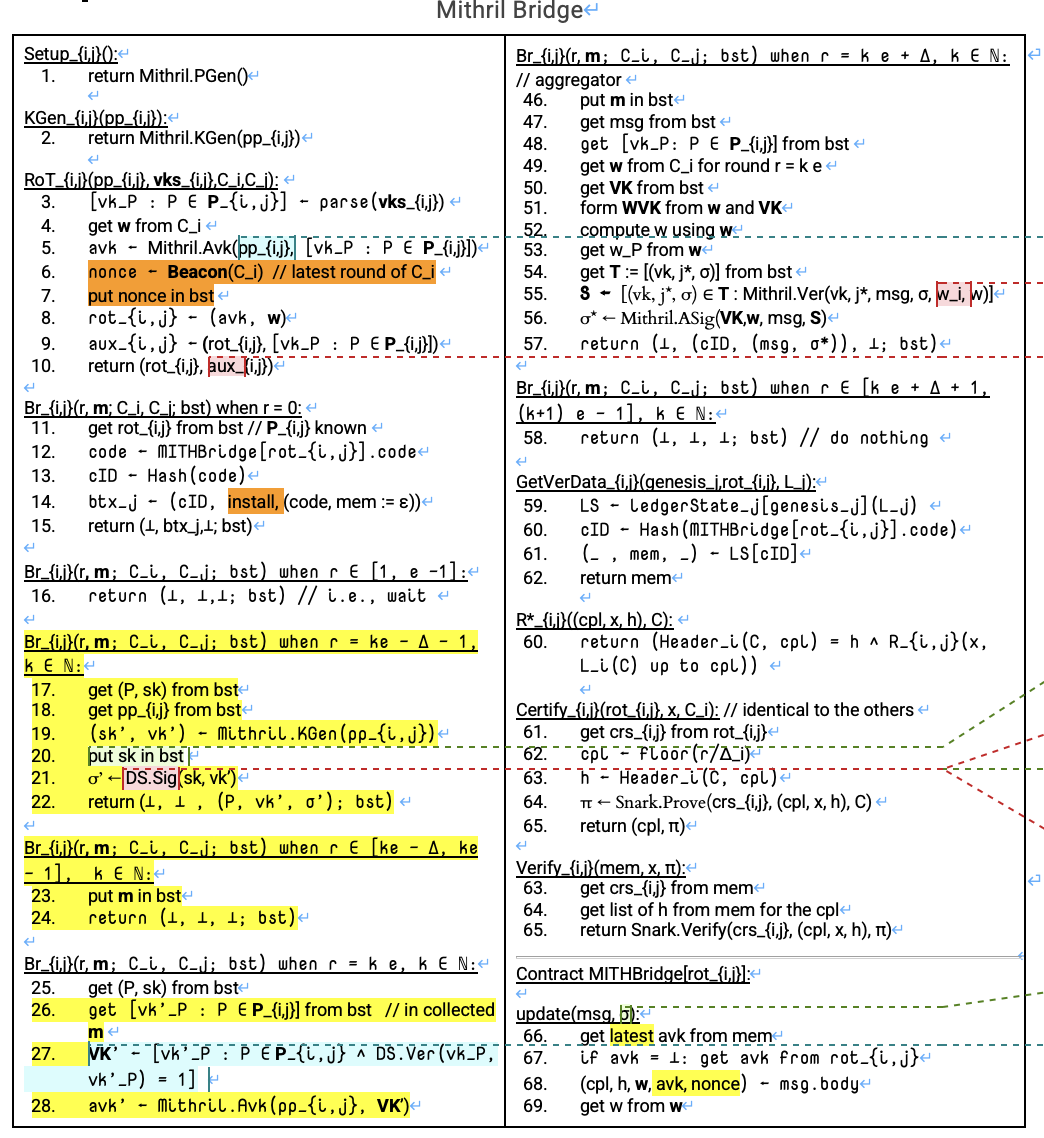
\includegraphics[width=1\linewidth]{截屏2025-08-26 15.16.55.png}
    % \caption{Enter Caption}
    \label{fig:placeholder}
\end{figure}

\begin{figure}
    \centering
    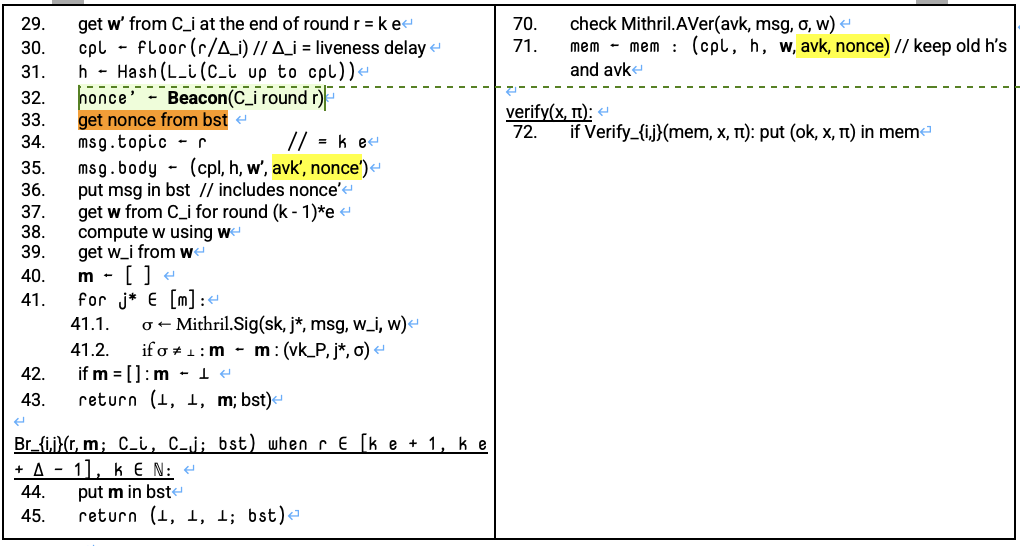
\includegraphics[width=1\linewidth]{截屏2025-08-26 15.18.40.png}
    % \caption{Enter Caption}
    \label{fig:placeholder}
\end{figure}








% \paragraph{Batch BLS Signature Aggregation (MSP.BSig)}
% \begin{align*}
% &e_{\sigma} \leftarrow H_p(\boldsymbol{\sigma}) \\
% &e_i \leftarrow H_\lambda(i, e_{\sigma}) \\
% &\mu \leftarrow \prod_i \sigma_i^{e_i} \\
% &\text{return } (\mu, e_{\sigma})
% \end{align*}



% \section{Benchmark Result on the New Server}

% \subsection{Server Configuration Information}


% The experiments were conducted on a G5500 V6 Whitley high-performance computing server, equipped with an Intel Xeon Platinum 8368 processor (2 cores @ 3.4GHz), 256GB of RAM, and running Ubuntu 22.04.5 LTS with kernel version 5.15.0-131-generic.




% \subsection{Benchmark Result}


% \textbf{Verification Relations for MSP.A:}
% \begin{itemize}
%   \item $\mathsf{MSP.AKey}(\mathbf{mvk})$ receives a set of verification keys $\mathbf{mvk}$ and computes the aggregate key $ivk = \sum_1^d mvk_i$.
%   \item $\mathsf{MSP.ASig}(\sigma)$ aggregates signatures as $\mu = \sum_1^d \sigma_i$.
%   \item $\mathsf{MSP.Ver}(msg, ivk, \mu)$ checks if $e(\mu, g_2) = e(H_{\mathbb{G}_1}(\text{``M''} \| msg), ivk)$.
% \end{itemize}

% \begin{table}[htbp]
% \centering
% \caption{Benchmark Results of $\mathsf{MSP.A}$}
% \renewcommand{\arraystretch}{0.9}
% \setlength{\tabcolsep}{10pt}
% \begin{tabular}{c|c|c|c|c|c|c} \toprule
%     \textbf{Aggregated sig num} & \textbf{2} & \textbf{200} & \textbf{2000} & \textbf{4000} & \textbf{6000} & \textbf{8000}  \\ \midrule 
%     Proof Time (s) & 19.17 & 29.51 & 72.89 & 123.67 & 181.38 & 226.84  \\ 
%     Proof Size (bytes) & 3072 & 4128 & 11424 & 18944 & 26944 & 34944  \\ 
%     Verification Time (ms) & 20.93 & 9.09 & 19.95 & 16.03 & 20.25 & 55.16 \\ \bottomrule 
% \end{tabular}
% \label{tab:mspa_benchamrk}
% \end{table}



% \textbf{Verification Relations for MSP.B:}
% \begin{itemize}
%   \item $\mathsf{MSP.BKey}(\mathbf{mvk}, \mathbf{e_\sigma})$ computes $ivk = \sum mvk_i^{e_i}$, where $e_i \leftarrow H_\lambda(i, \mathbf{e_\sigma})$.
%   \item $\mathsf{MSP.BSig}(\sigma)$ returns $(\mu, \mathbf{e_\sigma})$, with $\mu = \sum \sigma_i^{e_i}$.
%   \item $\mathsf{MSP.Ver}(msg, ivk, \mu)$ verifies $e(\mu, g_2) = e(H_{\mathbb{G}_1}(\text{``M''} \| msg), ivk)$.
% \end{itemize}


% \begin{table}[htbp]
% \centering
% \caption{Benchmark Results of $\mathsf{MSP.B}$}
% \renewcommand{\arraystretch}{0.9}
% \setlength{\tabcolsep}{10pt}
% \begin{tabular}{c|c|c|c|c|c|c} \toprule
%     \textbf{Aggregated sig num} & \textbf{8} & \textbf{16} & \textbf{32} & \textbf{64} & \textbf{128} & \textbf{256} \\ \midrule
%     Proof Time (s) & 35.73 & 48.48 & 65.37 & 103.75 & 184.02 & 327.30 \\ 
%     Proof Size (bytes) & 5856 & 7936 & 10944 & 17312 & 30240 & 55744 \\ 
%     Verification Time (ms) & 10.30 & 14.68 & 15.05 & 14.54 & 24.51 & 69.35 \\ \bottomrule
% \end{tabular}
% \label{tab:mspb_benchmark}
% \end{table}


% \newpage

% \textbf{Validation Relation:} For all $i$, $\mathsf{index}_i \leq m$ and for all $i \neq j$, $\mathsf{index}_i \neq \mathsf{index}_j$.



% \begin{table}[htbp]
% \centering
% \caption{Benchmark Results of Index Validation}
% \renewcommand{\arraystretch}{0.9}
% \setlength{\tabcolsep}{10pt}
% \begin{tabular}{c|c|c|c|c|c} \toprule
%     \textbf{Number of Index Checks} & \textbf{128} & \textbf{256} & \textbf{512} & \textbf{1024} & \textbf{2048}  \\ \midrule
%     Proof Time (s) & 4.08 & 6.77 & 13.41 & 37.39 & 122.49  \\ 
%     Proof Size (bytes) & 960 & 1920 & 4576 & 14944 & 14944  \\ 
%     Verification Time (ms) & 5.05 & 6.15 & 9.42 & 15.10 & 13.08  \\ \bottomrule
% \end{tabular}
% \label{tab:index_check_benchmark}
% \end{table}



% \textbf{Verification Relation:} For each $i \in \{1, \dots, k\}$,
% \[ \mathsf{MSP.Eval}(\mathsf{topic}, \mathsf{index}_i, \sigma_i) = ev_i \quad \text{and} \quad ev_i \leq \phi(\mathsf{stake}_i). \]


% \begin{table}[htbp]
% \centering
% \caption{Benchmark Results of Eligibility Check}
% \renewcommand{\arraystretch}{0.9}
% \setlength{\tabcolsep}{10pt}
% \begin{tabular}{c|c|c|c|c|c} \toprule
%     \textbf{Number of Checks} & \textbf{128} & \textbf{256} & \textbf{512} & \textbf{1024} & \textbf{2048}  \\ \midrule
%     Proof Time (s) & 10.14 & 12.78 & 17.36 & 26.39 & 44.56 \\ 
%     Proof Size (bytes) & 1344 & 1920 & 2848 & 4800 & 8832 \\ 
%     Verification Time (ms) & 6.77 & 6.39 & 7.10 & 11.24 & 12.59 \\ \bottomrule
% \end{tabular}
% \label{tab:eligibility_check_benchmark}
% \end{table}



\end{document}
